\newcount\draft\draft=0 % set to 0 for submission or publication
\documentclass[acmsmall,review,anonymous]{acmart}
\settopmatter{printfolios=true,printccs=false,printacmref=false}

% Remove some ACM template cruft for this draft/submission version.
\settopmatter{printfolios=true,printccs=false,printacmref=false}
\setcopyright{none}

\usepackage[utf8]{inputenc}
\usepackage{amsmath,amsthm,bbm,amsfonts,syntax,graphicx,tikz}
\usetikzlibrary{shapes,arrows, chains}
\usepackage[ligature, inference]{semantic}
\usepackage[T1]{fontenc}
\usepackage{mathpartir}
\usepackage{nccmath}
\usepackage{xspace}
\usepackage{xxx}
\usepackage{proof}
\usepackage{listings}
\lstset{escapeinside={<@}{@>}} % for color _coding_
\usepackage{booktabs} % for professional tables
\usepackage{subcaption}
\usepackage{bm}

\newcommand{\lang}{Gator\xspace}

\title{Geometry Types for Graphics Programming:
    \\ Supplementary Material}

\author{Dietrich Geisler}
\email{dag368@cornell.edu}
\author{Irene Yoon}
\email{ey222@cornell.edu}
\author{Horace He}
\email{hh498@cornell.edu}
\author{Aditi Kabra}
\email{ank55@cornell.edu}
\author{Yinnon Sanders}
\email{yys4@cornell.edu}
\author{Adrian Sampson}
\email{asampson@cs.cornell.edu}
\affiliation{%
  \institution{Cornell University}
  \city{Ithaca}
  \state{New York}
  \postcode{14853}
}
\date{}

% ACM publication cruft.
\acmJournal{PACMPL}
\acmVolume{1}
\acmNumber{OOPSLA}
\acmArticle{1}
\acmYear{2020}
\acmMonth{1}
\acmDOI{} % \acmDOI{10.1145/nnnnnnn.nnnnnnn}
\startPage{1}

% In draft mode, include git revision.
\ifnum\draft=1
\InputIfFileExists{revision}{}{\newcommand{\Revision}{}}
\subtitle{Draft \Revision}
\fancyfoot[LO,RE]{
  \footnotesize%
  Draft \Revision%
}
\fi

% Bibliography and citations.
\bibliographystyle{ACM-Reference-Format}
\citestyle{acmnumeric}

\newcommand{\mat}{\mathsf{mat}_{n_1{\times}n_2}}
\newcommand{\env}[1]{#1,\sigma}
\newcommand{\defas}{\mathrel{::=}}
\newenvironment{leftalign}%
{\fleqn[5pt]\csname align*\endcsname}%
{\csname endalign*\endcsname\endfleqn}
\newcommand{\alt}{\:|\:}
\newcommand{\bmark}{\textsf}

\mathlig{->}{\rightarrow}
\mathlig{|-}{\vdash}
\mathlig{=>}{\Rightarrow}

\tikzstyle{block} = [rectangle, draw, fill=gray!20,
text width=4em, text centered, rounded corners, minimum height=4em]
\tikzstyle{line} = [draw, -latex']

% Code listings configuration.
\lstdefinelanguage{GLSL}{
    keywords={vec4, vec3, vec2, mat3, mat4, void, float, int,
      if, abs, \#ifdef, \#else, \#endif, in, out, uniform,
      varying, attribute, return, void, space, is, coord, canon, type,
      declare, vec, mat, as, has, frame, object, dimension, coord},
    comment=[l]{//},
}
\lstset{
    language=GLSL,
    columns=fullflexible,
    keepspaces=true,
    showspaces=false,
    showstringspaces=false,
	keywordstyle=\bfseries,
	basicstyle=\ttfamily\small,
	basewidth=0.53em,
	aboveskip=0.9\medskipamount,
	belowskip=0.6\medskipamount,
	mathescape=true,
    lineskip={-2pt},
	% xleftmargin=\parindent,
}

% Shorthand for inline code.
\newcommand{\code}{\lstinline[keywordstyle=]}

% color definitions
\definecolor{darkolivegreen}{rgb}{0.33, 0.42, 0.18}

% Semantics declarations for the formalism.
\DeclareRobustCommand\tvdash{\mathrel{||}\joinrel\mkern-.5mu\mathrel{-}}
\newcommand{\source}[1]{\llbracket #1 \rrbracket}
\newcommand{\ld}[1]{\leq_\Delta}
\newcommand{\gen}[1]{\langle #1 \rangle} %generic
\newcommand{\sca}[0]{\textrm{scalar}}
\newcommand{\subsumption}{\textrm{SUBSUMPTION}}
\newcommand{\unit}{\textrm{UNIT}}
\newcommand{\scalar}{\textrm{SCALAR}}
\newcommand{\vect}{\textrm{VECTOR}} %both vec and vector lead to funky behavior
\newcommand{\matr}{\textrm{MATRIX}} %can't call this matrix because amsmath
\newcommand{\decl}{\textrm{DECL}}
\newcommand{\assign}{\textrm{ASSIGN}}
\newcommand{\add}{\textrm{ADDITION}}
\newcommand{\smul}{\textrm{SCAL MUL}}
\newcommand{\vmul}{\textrm{VEC MUL}}
\newcommand{\mmul}{\textrm{MAT MUL}}
\newcommand{\vcmul}{\textrm{VEC CMUL}}
\newcommand{\mcmul}{\textrm{MAT CMUL}}

\newcommand{\IH}{\textrm{I.H.}}
\newcommand{\TC}{\textrm{T.C.}}
\newcommand{\sub}{\textrm{SUBST}}

\newif\ifsemanticsdoc

\newtheorem{lemma}{Lemma}
\newtheorem{theorem}{Theorem}


\begin{document}
\renewcommand\thesection{\Alph{section}}
\setcounter{lemma}{0}
\maketitle

\section{GLSL Phong Source Code}
\label{app:llphong}

This section lists the full code for the Phong lighting model in plain GLSL~\cite{glsl}.

\begin{verbatim}
precision mediump float;

// External Function Declarations
uniform mat4 uModel;
uniform mat4 uView;
varying vec3 vNormal;
uniform vec3 uLight;
varying vec3 vPosition;

void main() {
  vec3 ambient = vec3(.1, 0., 0.);
  vec3 lightColor = vec3(0.4, 0.3, 0.9);
  vec3 specColor = vec3(1., 1., 1.);

  vec4 homWorldPos = uModel*vec4(vPosition, 1.0);
  vec3 camPos = normalize(vec3(uView*homWorldPos));
  vec3 worldNorm = 
	  normalize(vec3(uModel*vec4(vNormal, 0.0)));

  vec3 lightDir = 
    normalize(uLight - vec3(homWorldPos));
  vec3 reflectDir = reflect(lightDir, worldNorm);

  vec3 diffuse = 
    max(lightWorldDot, 0.0) * lightColor;

  float spec = pow(max(-dot(
    camPos, reflectDir), 0.), 32.);
  vec3 specular = spec * specColor;

  gl_FragColor = vec4(ambient+diffuse+specular, 1.0);
}
\end{verbatim}

\section{\lang Phong Source Code}
\label{app:hlphong}

This section lists equivalent code in \lang.

\begin{verbatim}
#"precision mediump float;";
using "../glsl_defs.lgl";

// Reference Frame Declarations

frame model has dimension 3;
frame world has dimension 3;
frame camera has dimension 3;
frame light has dimension 3;

// Global Variables

varying cart3<model>.point vPosition;
canon uniform hom<model>.transformation<world> uModel;
canon uniform hom<world>.transformation<camera> uView;
varying cart3<model>.vector vNormal;
uniform cart3<light>.point uLight;
canon uniform hom<light>.transformation<world> uLightTrans;

// Shader Code

void main() {
  color ambient = [.1, 0., 0.];
  color diffColor = [0.4, 0.3, 0.9];
  color specColor = [1.0, 1.0, 1.0];

  auto worldPos = vPosition in world;
  auto camPos = worldPos in camera;
  auto worldNorm = normalize(vNormal in world);

  auto lightDir = normalize((uLight in world) - worldPos);
  auto lightWorldDot = dot(lightDir, worldNorm);
  scalar diffuse = max(lightWorldDot, 0.0);

  auto reflectDir = normalize(reflect(-lightDir, worldNorm) in camera);

  scalar specular = pow(max(dot(normalize(-camPos), reflectDir), 0.), 32.);

  vec4 gl_FragColor = 
    vec4(ambient + diffuse * diffColor + specular * specColor, 1.0);
}
\end{verbatim}

\section{Case Study Images}

\begin{figure}
	\centering
	\begin{subfigure}[b]{0.45\linewidth}
		\centering
		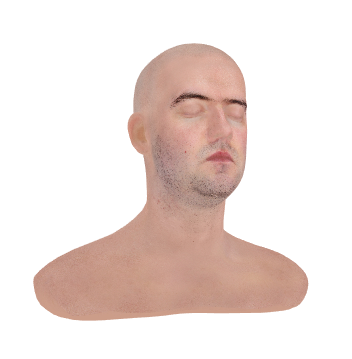
\includegraphics[width=\linewidth]{fig/texture.png}
		\caption{Texture.}
	\end{subfigure}
	\hfill
	\begin{subfigure}[b]{0.45\linewidth}
		\centering
		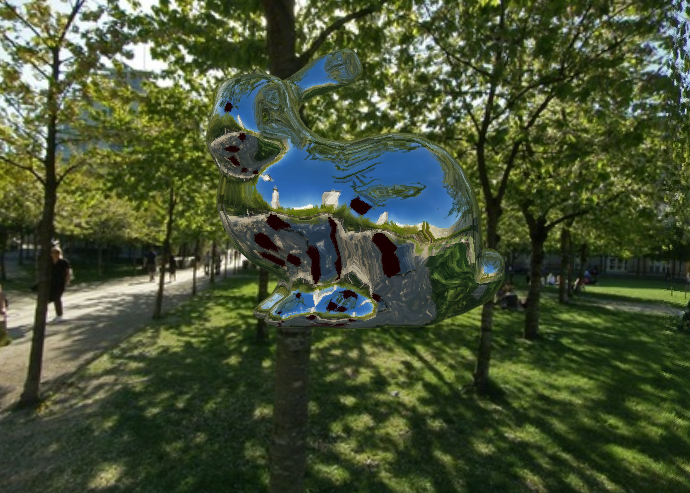
\includegraphics[width=\linewidth]{fig/reflection.png}
		\caption{Reflection.}
	\end{subfigure}
	
	\begin{subfigure}[b]{0.45\linewidth}
		\centering
		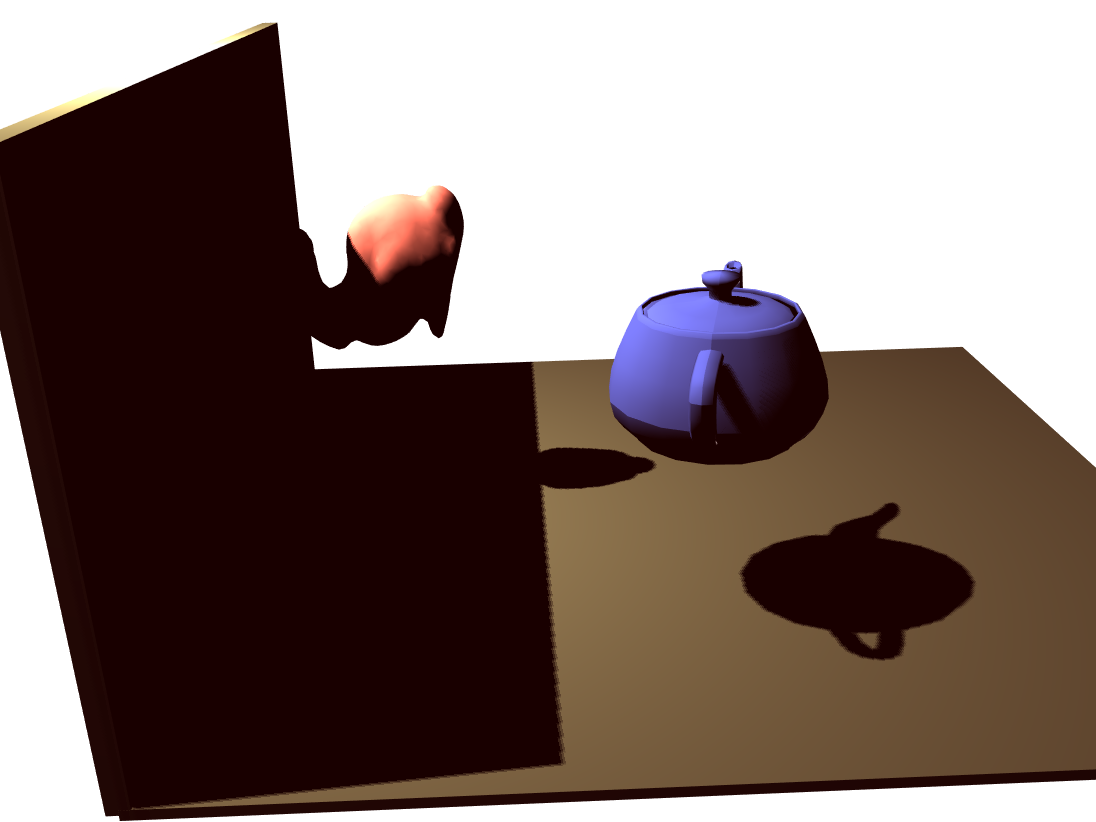
\includegraphics[width=\linewidth]{fig/shadowmap.png}
		\caption{Shadow map.}
	\end{subfigure}
	\hfill
	\begin{subfigure}[b]{0.45\linewidth}
		\centering
		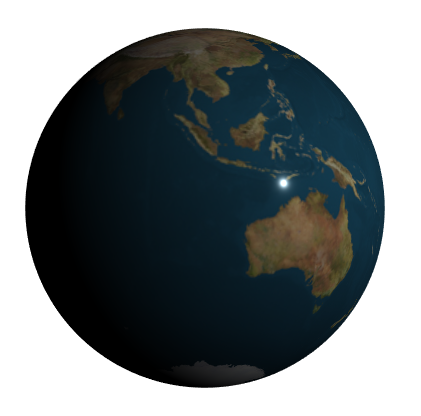
\includegraphics[width=\linewidth]{fig/microfacet.png}
		\caption{Microfacet.}
	\end{subfigure}
	\caption{Example outputs from first four renderers used in our case studies.}
\end{figure}
\begin{figure}
		\begin{subfigure}[b]{0.45\linewidth}
		\centering
		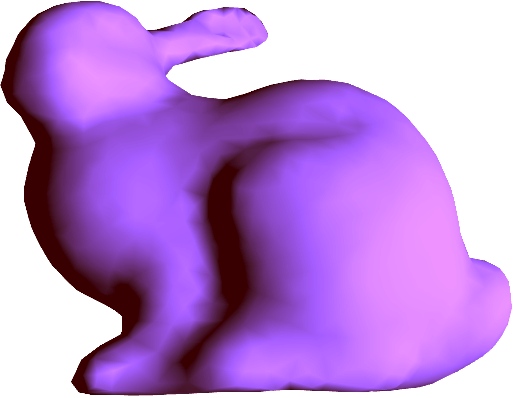
\includegraphics[width=\linewidth]{fig/bunnygoodfront.png}
		\caption{Phong}
	\end{subfigure}
	\hfill
	\begin{subfigure}[b]{0.45\linewidth}
		\centering
		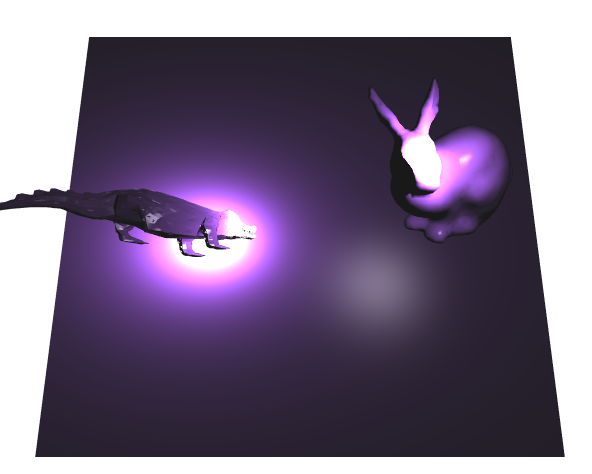
\includegraphics[width=\linewidth]{fig/fog.png}
		\caption{Fog}
	\end{subfigure}
		\begin{subfigure}[b]{0.45\linewidth}
		\centering
		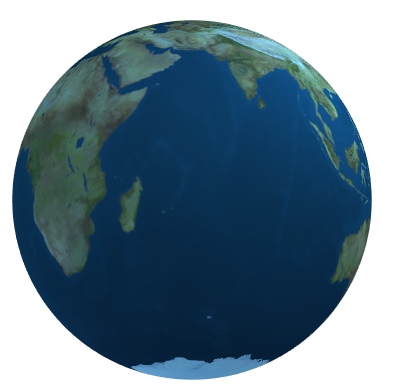
\includegraphics[width=\linewidth]{fig/bump.png}
		\caption{Bump Map}
	\end{subfigure}
	\hfill
	\begin{subfigure}[b]{0.45\linewidth}
		\centering
		
\includegraphics[width=\linewidth]{fig/spotlight.png}
		\caption{Spotlight}
	\end{subfigure}
	\caption{Example outputs from last four renderers used in our case studies.}
\end{figure}

\section{Full Formal Semantics}
\label{app:formalism}
\subsection{\lang's Syntax}
\semanticsdocfalse

\subsubsection{Type System}

\begin{gather*}
c \in\text{constants}\\
x \in\text{variables}\\
p \in\text{primitives}\\
t \in\text{types} \\
\tau \defas \textrm{unit} \,|\, \top_p \,|\, \bot_p \,|\, t \\
f \in \text{function names} \\ 
\ifsemanticsdoc
    Only binary functions are modeled in this document, however their treatment can be easily generalized to functions with an arbitrary number of inputs.
\fi
e \defas x \,|\, c \,|\, f(e_1, e_2) \,|\, x\ \textrm{as!}\ \tau \,|\, x\ \textrm{in}\ \tau\\
C \defas \tau \, x = e \,|\, e \\
P  =  C;P \,|\, \epsilon 
\end{gather*}

\subsection{\lang's static rules}

  \begin{mathpar}
	\inferrule
	{\tau_1\leq\tau_2\qquad\Gamma\vdash e:\tau_1}
	{\Gamma\vdash e:\tau_2}
	
	\inferrule
	{\textrm{X}(c)=p}
	{\Gamma\vdash c:\bot_p}
	
	\inferrule
	{\Gamma(v)=\tau}
	{\Gamma\vdash x :\tau}
	
	\inferrule
	{\Gamma\vdash e : \tau\qquad\Gamma(v)=\tau}
	{\Gamma\vdash \tau\ x = e:\textrm{unit}}
	
	\inferrule
	{\Gamma\vdash C : \tau_1\qquad\Gamma\vdash P : \tau_2}
	{\Gamma\vdash C;P:\textrm{unit}}
	
	\inferrule
	{ }
	{\Gamma\vdash \epsilon:\textrm{unit}}
	
	\inferrule
	{\Gamma\vdash e: \top_p\qquad\tau\leq\top_p}
	{\Gamma\vdash e\ \textrm{as!}\ \tau:\tau}
	
	\inferrule
	{\Gamma\vdash e : \tau_1\qquad\textrm{P}(\tau_1,\tau_2)=f}
	{\Gamma\vdash e\ \textrm{in}\ \tau_2:\tau_2}
	
	\inferrule
	{\Gamma\vdash e_1:\tau_1\qquad\Gamma,\vdash e_2:\tau_2 \qquad \Phi(f,\tau_1,\tau_2)=\tau_3}
	{\Gamma\vdash f(e_1,e_2):\tau_3}
\end{mathpar}
\label{fig:semantics}


\subsection{Ordering rules}
\begin{mathpar}
\inferrule
{ }
{\tau\leq\tau}

\inferrule
{\tau_1 \leq \tau_2 \and \tau_2 \leq \tau_3}
{\tau_1 \leq \tau_3}

\inferrule
{ }
{\tau\leq\mathsf{unit}}

\inferrule
{ }
{\bot_p\leq\top_p}

\inferrule
{\tau\leq\top_p}
{\bot_p\leq\tau}
\end{mathpar}
\label{fig:subtype}

\subsection{Target language grammar}
Hatchling is an abstraction over sound imperative languages.

It has an \textit{operation context} $\Xi$ that maps operator names and types to their implementation. $\Xi : (\textrm{operator names}), \tau_1, \tau_2 \rightarrow \textrm{type}$.

We use the symbol $\tvdash$ for judgment in the target language

\subsubsection{Hatchling's syntax}
\begin{gather*}
c \in\textrm{constants}\\
x \in\textrm{variables}\\
p\in\textrm{primitives}\\
t\in\textrm{types}\\
\tau ::= \textrm{unit} \,|\, \top_p \,|\, \bot_p \\
o \in \textrm{operation names} \\
e ::= x \,|\, c \,|\, o(e_1, e_2) \\
c ::= \tau \, x = e\,|\, e \\
P  =  c;P \,|\, \epsilon 
\end{gather*}

\subsubsection{Hatchling's static semantics}
Subsumption
\begin{mathpar}
\infer[\subsumption]{\Gamma \tvdash e:\textrm{unit}, \Gamma}{\Gamma \tvdash e: \tau,\Gamma}
\end{mathpar}

Constants and variable declarations

\begin{mathpar}
 \infer[UNIT]{\Gamma \tvdash ():\textrm{unit}}{}
\end{mathpar}
\begin{mathpar}
\infer[VAR]
{\Gamma\vdash v:\tau}
{\Gamma\vdash \Gamma(v)=\tau}
\end{mathpar}
\begin{mathpar}
 \infer[PRIMITIVE]{\Gamma\vdash c:\bot_\mathsf{p}}{\Gamma\vdash X(c)=p} 
\end{mathpar}
\begin{mathpar}
 \infer[DECL]{\Gamma \tvdash \tau x:=e:\textrm{unit}, x\mapsto \tau}{\Gamma\tvdash e:\tau}
\end{mathpar}

Operations

\begin{mathpar}    
\infer[OP]
{\Gamma\vdash o(e_1,e_2):\tau_3}
{\Gamma\vdash e_1:\tau_1\qquad\Gamma,\vdash e_2:\tau_2 \qquad \Gamma\vdash \Xi(o, \tau_1, \tau_2)=\tau_3} 
\end{mathpar}


\subsection{Translation}

\subsubsection{Literals}
\begin{gather*}
\source{c} \triangleq c
\end{gather*}

\subsubsection{Types}
\begin{gather*}
\source{T} \triangleq \top_p \\
\text{Where we know $\top_n$ is always defined because of the structure imposed on a well formed $\Delta$.}\\
\source{\top_p} \triangleq \top_p \\
\source{\bot_p} \triangleq \top_p \\
\source{\textrm{unit}} \triangleq \textrm{unit} \\
\end{gather*}

\subsubsection{Expressions}
\begin{align*}
\source{c}_\Gamma &\triangleq c \\
\source{x}_\Gamma &\triangleq x \\
\source{\tau\ x := e}_\Gamma &\triangleq \source{\tau}\ x := \source{e}_\Gamma \\
\source{e\ \mathrm{as!}\ \tau}_\Gamma&\triangleq \source{e}_\Gamma \\
\source{e\ \mathrm{in}\ \tau_2}_\Gamma&\triangleq \source{f(e)}_\Gamma&\text{where }&\Gamma|-e:\tau_1\text{ and }f=\mathrm{P}(e,\tau_1,\tau_2)\\
\source{f(e_1, e_2)}_\Gamma&\triangleq f'(e_1, e_2)&\text{where }&\Gamma|-e:\tau_1,\Gamma|-e:\tau_2,\text{ and }f'=\Psi(f,e_1,e_2,\tau_1,\tau_2)\\
\source{\epsilon}_\Gamma&\triangleq \epsilon\\
\source{C;P}_\Gamma&\triangleq\source{C}_\Gamma;\source{P}_\Gamma\\
\end{align*}

\subsubsection{}
Additionally, we define the translation of $\Gamma$ and $\Phi$; in the target language, we replace every $\tau$ in the range of $\Gamma$ and $\Phi$ with its translation to get $\source{\Gamma}$ and $\source{\Phi}$. This is a different translation function than the one previously discussed, but for convenience we will use the same notation $\source{\Gamma}$ and $\source{\Phi}$.\\
\begin{lemma}
\label{lem:contexttr}
\begin{mathpar}
    \infer[]{
            \source{\Gamma} \tvdash \source{\Gamma}(\source{x}_\Gamma):\source{\tau}}{
                  {\source{\Gamma \vdash \Gamma(x) : \tau}_\Gamma}
        }
\end{mathpar}
\begin{mathpar}
    \infer[]{
            \source{\Gamma} \tvdash \source{\Gamma}(\source{\Phi(f, \tau_1, \tau_2)}_\Gamma):\source{\tau}}{
                  {\source{\Gamma \vdash \Phi(f, \tau_1, \tau_2) : \tau_3}_\Gamma}
        }
\end{mathpar}
\end{lemma}

\begin{proof}
Follows from the definitions of $\source{\Gamma}$ and $\source{\Phi}$.
\end{proof}

\subsection{Proof that if source type checks then translation type checks}
We use structural induction over \lang commands to show that any translation under a valid $\Delta$ type checks.
In the process of the induction we use the theorem that if a \lang expression type checks then its translation does too. This is also shown using structural induction over all \lang expressions.
\begin{theorem}
    Given any \lang expression $e$ that type checks under some $\Gamma$ to produce $\tau$, we prove that its translation $\source{e}$ also type checks under $\source{\Gamma}$ to produce $\source{\tau}$.
\end{theorem}
\begin{theorem}
	Given any \lang program $P$ that type checks under some $\Gamma$ to produce $\tau$, we prove that its translation $\source{e}$ also type checks under $\source{\Gamma}$ to produce $\source{\tau}$.
\end{theorem}
Below, I.H. = Inductive Hypothesis. Sometimes the inductive hypothesis is used over a general $\tau$. This implicitly excludes the special case of the polymorphic type.\\
We use the inversion of the type checking rules in \lang; if a statement in \lang type checks then we know that the premise of the corresponding type checking rule is true. Using this rule will be marked as T.C. \\

We split the proof into cases, one for each of the typing judgement rules in \lang.

\subsubsection{Expressions Type Check}

We present the most interesting case, for primitives. The other cases follow vry similarly.

\paragraph{Primitive rule}
\begin{mathpar}
    \inferrule*[Right=\sub]{
    \inferrule*[right=PRIM]{ }{\source{\Gamma}\tvdash c:\top_p,\source{\Gamma}} \\
    \source{\top_p} \triangleq \top_p \\
    \source{c}\triangleq c }
    {\source{\Gamma}\tvdash\source{c}:\source{\top_p}}
\end{mathpar}

Functions type check because of the constraints on a well formed $\Psi$.

\begin{mathpar}
    \inferrule*[Right=\sub]{
    \inferrule*[]{\Gamma\vdash f(e_1 : \tau_1, e_2 : \tau_2):\tau_3 }{\Phi(f, \tau_1, \tau_2) = \tau_3} \\
    \source{\Gamma}\tvdash\Psi(f, e_1, e_2, \tau_1, \tau_2) = \source{\Phi(f, \tau_1, \tau_2)}}
    {\source{\Gamma}\tvdash\source{f(e_1 : \tau_1, e_2 : \tau_2)}:\source{\tau_3}}
\end{mathpar}


\subsubsection{Commands Type Check}

\subsubsection{Declaration}
One case is presented here, and other follows suit along the same lines.
\paragraph{Declaration}
\small{
\begin{mathpar}
%\hspace*{-1.2cm}
\infer[\sub]{  %leaving this as \infer to force inlining, which doesn't seem to happen with \inferrule
    \source{\Gamma} \tvdash \source{\tau x := e}:\source{\textrm{unit}}, \source{\Gamma, x\mapsto\tau}}{
    {\inferrule*[Right=\sub]{
        \inferrule*[Right=\decl]{
            \inferrule*[Right=\IH]{
                    \inferrule*[Right=\TC]{
                        \source{\Gamma\vdash\tau x:=e:\textrm{unit},x\mapsto\tau}
                    }
                    {\source{\Gamma \vdash e : \tau}}
                }
                {\source{\Gamma} \tvdash \source{e}:\source{\tau}}
            } 
            {\source{\Gamma} \tvdash \source{\tau} \source{x} := \source{e} :\textrm{unit}, \source{x}\mapsto\source{\tau}} \\
        \source{\tau x := e} \triangleq ...
        }
        {\source{\Gamma} \tvdash \source{\tau x := e}:\textrm{unit}, \source{\Gamma}, \source{x}\mapsto\source{\tau}}} 
    \source{\Gamma, x\mapsto \tau} \triangleq 
    \source{\Gamma}, \source{x}\mapsto \source{\tau} 
    \source{\textrm{unit}} \triangleq \textrm{unit}
    }
\end{mathpar}
}


\bibliography{venues,refs}

\end{document}
